\chapter{Conclusions and Future Work}\label{ch:conclusions}

This thesis presents a \acrshort{dt} for smart homes that can forecast and optimize the energy consumption of various appliances in a hypothetical smart home. The appliances were chosen from the GREEND and UK-DALE datasets, which were selected among the power consumption datasets in the literature for their relevance and quantity of data.

The appliances are assumed to have a set of operation modes with different energy consumptions, and they can be set to operate in a specific mode at a given time through user-created routines. The operation modes of the appliances were inferred using a hybrid \acrshort{ml} and the manufacturers' manuals. 

The \acrshort{dt} was implemented as a \acrshort{rest} \acrshort{api}, which offers several endpoints to access information about appliances, routines, and consumptions. The \acrshort{api} also enables simulating the addition of new routines and provides feedback about errors and context-aware recommendations. A frontend application was developed to showcase the functionalities of the \acrshort{dt}.

Future work should focus on making the system more comprehensive and usable. The following are some of the possible improvements and extensions that could be made to the \acrshort{dt}:
\begin{description}
    \item[Physical twin.] The \acrshort{dt} developed in this thesis is a digital-only system that cannot interact with the physical world directly. To enable this interaction, it needs to connect to the smart devices in the home and send commands to them. This entails developing a physical twin similar to the hypothetical home presented in Chapter~\ref{ch:hypothetical_home}. The \acrshort{dt} should also update the state of the devices and the energy consumption according to the changes in the physical world.

    \item[Appliance data.] Future versions of the \acrshort{dt} should let users add new appliances by automatically importing their consumption values and operation modes. This requires having a list of smart devices that are compatible with the \acrshort{dt}, and whose data are accessible during the system configuration. Since the appliance data format is custom, it may be necessary to use a standardized format for the data or develop a system that can automatically convert the data from the appliance to the format used by the \acrshort{dt}. These consumption values should be treated as approximate and based on the new and optimal functioning of the appliance. Over time, the \acrshort{dt} should learn from the actual consumption, as they may vary due to malfunctions or lack of maintenance.

    The \acrshort{dt} could also work with non-smart appliances that do not provide information about themselves, by using a \acrshort{ml} approach similar to the one used in Chapter~\ref{ch:hypothetical_home} to automatically detect the operation modes and consumptions.

    \item[Manual appliance activation.] The \acrshort{dt} should be able to handle the manual activation of appliances by end users, by automatically detecting their state changes and resolving conflict C3 (see Section~\ref{sec:simulation}). Moreover, the \acrshort{dt} could monitor the manual activations of appliances and their duration, and use this information to provide suitable recommendations to automate the activations or modify existing routines. For instance, if the user starts the computer every day at 9:00, the \acrshort{dt} could propose to automate this activation. If the computer stays on for 8 hours on average, the \acrshort{dt} can use this information to anticipate whether this could cause any conflict with existing routines, and avoid them before they occur.

    \item[Predictions over multiple days.] Currently, the \acrshort{dt} can only predict the energy consumption for the current day. Future versions should enable the system to predict the energy consumption for several days ahead, and also view the consumption history for the previous days. This would allow the system to provide more precise recommendations, and to better handle the conflicts between routines. For example, if the user is planning to go on vacation for a week, the \acrshort{dt} could advise to set the boiler to the \textit{holiday} mode, and to turn off the fridge.

    \item[Multiple users.] A future enhancement for the \acrshort{dt} is to support multiple users in the home. This would require an authentication scheme to protect the \acrshort{dt} from unauthorized access, and to assign different roles and permissions to users. This would be useful for a family, where the children have limited control over the routines, and can only create new ones with certain restrictions. For example, they may not be allowed to create routines that involve the dishwasher or the washing machine, and they may have a time limit for using the TV.\@ The parents, on the other hand, may have full control over the system and could also monitor the children's activities.

    Multiple users for the \acrshort{dt} also pose a new challenge of resolving conflicts, which occur when a user creates a routine whose actions clash with those of a routine created by another user. For instance, a user may create a routine to set the AC to \textit{heat} from 10:00 to 12:00, while another user already created a routine to set it to \textit{cool} from 9:00 to 12:00. These conflicts may be handled in several ways, such as by giving priority to the user with the highest role, preferring the routine that was created first, or by asking the users to resolve the conflict manually.

    \item[Frontend.] To allow the end users to interact with the \acrshort{dt} effectively and also consider the future developments, a more comprehensive frontend application than the showcase one developed in this thesis is required. A frontend application for Android devices that meets these requirements is currently being developed as part of the broader research project.
\end{description}

The work discussed in this thesis contributed to an article submitted to the ACM International Conference on Advanced Visual Interfaces (AVI '24) with the following name: ``Barbara Rita Barricelli, Luca Cotti, Daniela Fogli, Davide Guizzardi, Matteo Pigoli.\ \textit{A Digital Twin to Enhance Energy Consumption Awareness in a Smart Home}''.

\vspace*{\fill} % Spazio bianco per mettere il testo in fondo alla pagina

\begin{figure}[h]
    \centering
    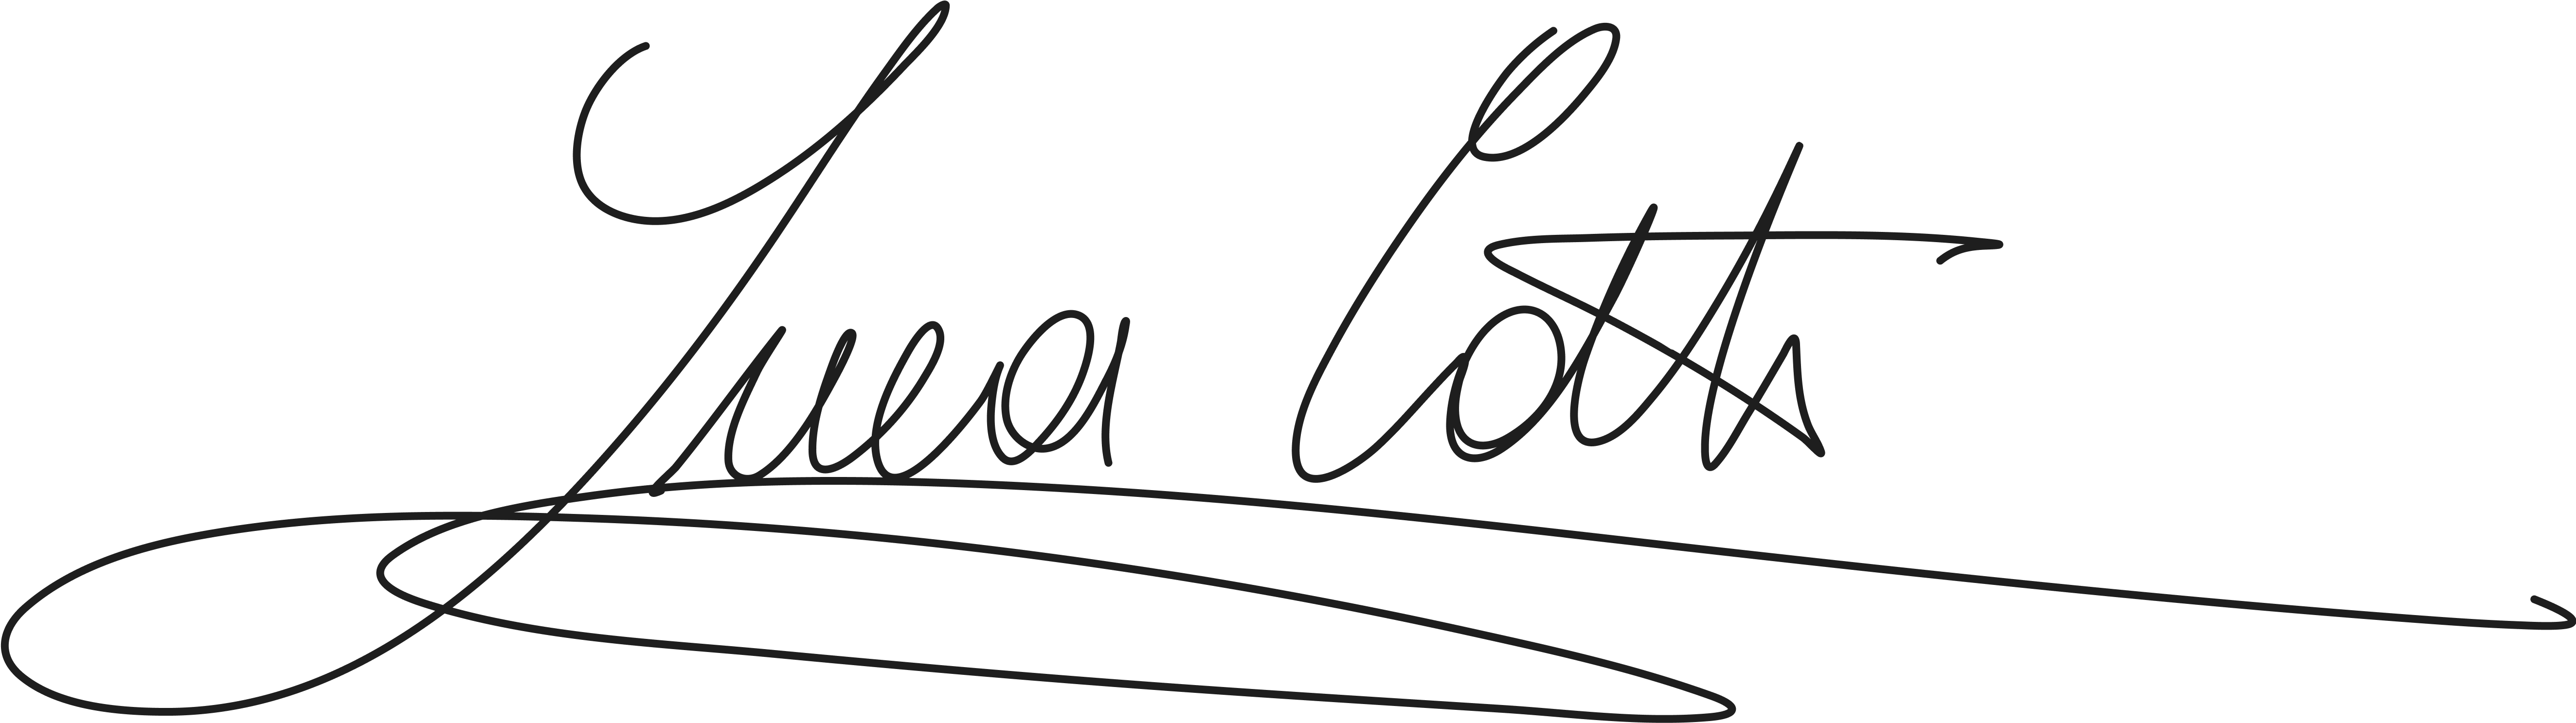
\includegraphics[width=.6\textwidth]{images/signature.png}
\end{figure}

\vspace*{16mm} % Spazio bianco per mettere il testo in fondo alla pagina